\documentclass[10pt,a4paper]{article}
\usepackage[margin=2cm]{geometry}
\usepackage{amsmath,amssymb,booktabs,graphicx,caption,xcolor,float,hyperref,tikz}
\usetikzlibrary{arrows.meta,positioning,calc}
\hypersetup{colorlinks=true,linkcolor=blue!50!black,urlcolor=blue!50!black}
\captionsetup{font=small,labelfont=bf}
\title{\vspace{-1.2cm}\textbf{Steering a swarm that owns a proof}\\[2pt]
\large Simulation 1 (days and nights), setup \texttt{task003-symmetric}}
\author{LLM-free simulator; report of 15 October 2026; runs of 15 October 2026\\
\small Mirrors the Simulation 2 report of the same date: same sections, figures and equations.}
\date{}
\begin{document}
\maketitle
\vspace{-1cm}

\paragraph{How the simulator works.} The world, \texttt{task\_003}, has three candidate allocations; A0 is the
correct one. Each of 24 agents is given one true fact and reasons as an exact Bayesian: its \emph{belief} is the
exact probability of A0, A1 and A2 given the facts it currently remembers. An episode has 30 rounds, each a day
and a night. During the day the agents act one at a time in a new random order: an agent reads $q$ posts drawn at
random from a shared \emph{board} (never its own), adds their facts to its memory, recomputes its belief,
\emph{votes} by probability matching (a vote drawn from its belief) and posts one remembered fact that supports
its vote. At night a \emph{controller} with a target, A0 (truth) or A2 (false), reads $q_c$ agent posts and,
unless the \emph{vote gate} (at least 75\% of them from agents voting for its target) or the \emph{proof stop}
(what it read already proves its target) silences it, posts the $b$ facts from its pool that best support its
target. The board is then cleared, keeping only the controller's new posts. At each dawn every remembered fact is
forgotten with probability $1-\rho$ and comes back if read again. Every episode is run three times with the same
random draws: without a controller (\emph{silent}), with the controller targeting A0 and with the one targeting
A2.

\paragraph{The facts at the start.} All facts are true. The agents hold, together, a proof of A0; no single
agent does, and neither pool can prove its target (Table~\ref{tab:facts}).

\begin{table}[H]
\centering\small
\caption{Facts available at the start and what each set implies, $P(\text{A0}, \text{A1}, \text{A2} \mid \text{facts})$.}
\label{tab:facts}
\begin{tabular}{lcc}
\toprule
set of facts & facts & $P(\text{A0}, \text{A1}, \text{A2})$ \\
\midrule
agents' facts, all together (24 agents, one fact each) & 18 distinct & (1, 0, 0): proves A0 \\
A0 pool (controller with target A0) & 12, of which 10 new to the agents & (0.963, 0.037, 0) \\
A2 pool (controller with target A2) & 12, of which 10 new to the agents & (0.114, 0, 0.886) \\
agents' facts + either pool & 28 distinct & (1, 0, 0) \\
\bottomrule
\end{tabular}
\end{table}

\paragraph{The runs.} Posts read by an agent $q \in \{3, 6, 12\}$; posts read by the controller
$q_c \in \{3, 6, 12, 24\}$; facts posted per night $b \in \{1, \dots, 9\}$ (at most 12, the pool size); memory
$\rho \in \{1, 0.75, 0.5, 0.25\}$; vote gate on and off; proof stop on; 1{,}000 episodes per setting (1{,}740
settings). Unless stated otherwise: $q = 6$, $q_c = 12$, $b = 1$ (the main setting, which posts about as many
facts as Simulation 2 at rate 1), gate on. Gate-off results are in Appendix~\ref{app:gateoff}.

\paragraph{Summary.} The 24 agents together own a proof of A0, and with full memory they keep it: no controller
changes the swarm for more than a few days. \textbf{Forgetting is what makes the swarm steerable}, and in this
simulation the effect peaks at intermediate memory: at $\rho = 0.5$ the false controller raises the share voting A2
by 0.53--0.57 and wins 78\% of the votes, against 0.31--0.36 at $\rho = 0.25$ and 0.22--0.58 at $\rho = 0.75$
(Figures~\ref{fig:votes}, \ref{fig:gaintime}). \textbf{The budget matters only when agents remember well}: at
$\rho \le 0.5$ one fact per night achieves almost everything, and it is five to seven times more effective per
fact than nine (Figures~\ref{fig:strength}, \ref{fig:perfact}). \textbf{Reading more posts protects the proof when agents
remember, and helps the controller when they forget} (Figure~\ref{fig:phasegain}c). Every controller replaces part of
the agents' own proofs (Figure~\ref{fig:proofs}). The target is most readable at $\rho = 0.5$ (0.42--0.49 bits from
one vote); the efficiency $\eta$ is 0.56--0.91 and is lowest where the two controllers are most unequal
(Figures~\ref{fig:Itime}--\ref{fig:phaseeta}). Turning the vote gate off adds 43--98 facts per episode and up to 0.16
in susceptibility (Appendix~\ref{app:gateoff}). Swarm-level states read up to five times more than one vote, with
a lower efficiency (Appendix~\ref{app:states}).

\section{Quantities}\label{sec:quantities}

\paragraph{Votes.} With $n_{a,t}$ the number of agents whose vote on day $t$ is answer $a$ and $N_t = 24$ (every
agent votes every day; before the first day nobody has voted and we set $x_{a,0} = 0$),
\begin{equation}\label{eq:share}
x_{a,t} = n_{a,t}/N_t .
\end{equation}

\paragraph{Paired susceptibility.} Following \texttt{BLACKBOARD\_OBSERVABLES\_AND\_EFFICIENCIES} (\S3), for a
controller policy $\pi$ and an answer $a$,
\begin{equation}\label{eq:chi}
\chi^{(a)}_{\pi,t} \equiv G^{(a)}_t(\pi) = \mathbb E\bigl[x^{\pi}_{a,t} - x^{\rm base}_{a,t}\bigr],
\end{equation}
the mean over episodes of the difference between the controlled run and the silent run of the same episode. We
report it on the controller's own target: $G_t \equiv G^{(0)}_t(\pi^{+})$ for the controller targeting A0 and
$G_t \equiv G^{(2)}_t(\pi^{-})$ for the one targeting A2.

\paragraph{Target and state.} The target $Z \in \{\text{A0}, \text{A2}\}$ is drawn by a fair coin. The state $X$
of the swarm on day $t$ is one of:
\begin{itemize}\itemsep1pt
\item \textbf{one agent's vote} (main text): the vote of a randomly chosen agent, $X \in \{\text{A0},\text{A1},\text{A2}\}$;
\item \textbf{plurality}: the answer with the most votes (a $k$-way tie gives $1/k$ to each);
\item \textbf{S1}: the agents' mean belief in A0, $m_{\text{A0}}$, cut at 0.33, 0.50 and 0.75 (4 values);
\item \textbf{S3}: $(m_{\text{A0}}, m_{\text{A2}})$, each cut into thirds of $[0, 1]$ (9 values, 6 reachable).
\end{itemize}
Each episode $e$ of arm $s$ (silent 0, target A0 $+$, target A2 $-$) gives a probability vector $y^{(e)}_s$ over
the values of $X$ (for one agent's vote, the episode's vote shares; for the others, a mark on one value), and
\begin{equation}\label{eq:P}
P_s(x) = \frac1E\sum_{e=1}^{E} y^{(e)}_s(x), \qquad E = 1000 .
\end{equation}

\paragraph{Readability and efficiency.} With $Q = \frac12(P_+ + P_-)$ and $\mathrm{KL}(p\Vert q) = \sum_x p(x)\log_2[p(x)/q(x)]$,
\begin{equation}\label{eq:I}
I(Z;X) = \tfrac12\,\mathrm{KL}(P_+\Vert Q) + \tfrac12\,\mathrm{KL}(P_-\Vert Q),
\end{equation}
the information the state carries about the target (at most 1 bit). The controllers' total change from silence
splits exactly into a directed and an undirected part,
\begin{equation}\label{eq:C}
C = \tfrac12\,\mathrm{KL}(P_+\Vert P_0) + \tfrac12\,\mathrm{KL}(P_-\Vert P_0) = I(Z;X) + \mathrm{KL}(Q\Vert P_0),
\end{equation}
and the efficiency is the directed share,
\begin{equation}\label{eq:eta}
\eta = I(Z;X)/C .
\end{equation}
Silence sometimes never shows a value of $X$ that a controller reaches, which would make $C$ infinite. Before
computing any KL, every arm's distribution therefore receives the same pseudo-count of $\alpha = 0.5$ episodes per
value of $X$ ($K$ values),
\begin{equation}\label{eq:smooth}
\tilde P_s(x) = \frac{E\,P_s(x) + \alpha}{E + \alpha K}.
\end{equation}
With $\alpha = 1$ instead, $\eta$ changes by at most 0.004 for one agent's vote and 0.06 for the other states; where
$C$ is finite without smoothing, by at most 0.014. $\eta$ is not defined when $C < 0.01$ bits (no measurable change);
such values are left blank. Equation~(\ref{eq:C}) holds in the data to $4\times10^{-15}$ bits.

\paragraph{Cost.} $F_t$ is the number of facts the controller has posted on the nights before day $t$ (mean per
episode); the gain per fact is $G_t/F_t$, and the marginal susceptibility is the slope between neighbouring
budgets,
\begin{equation}\label{eq:slope}
\frac{\Delta G}{\Delta b} = \frac{G(b^{(k+1)}) - G(b^{(k)})}{b^{(k+1)} - b^{(k)}} .
\end{equation}

\section{Votes over time}

\begin{figure}[H]
\centering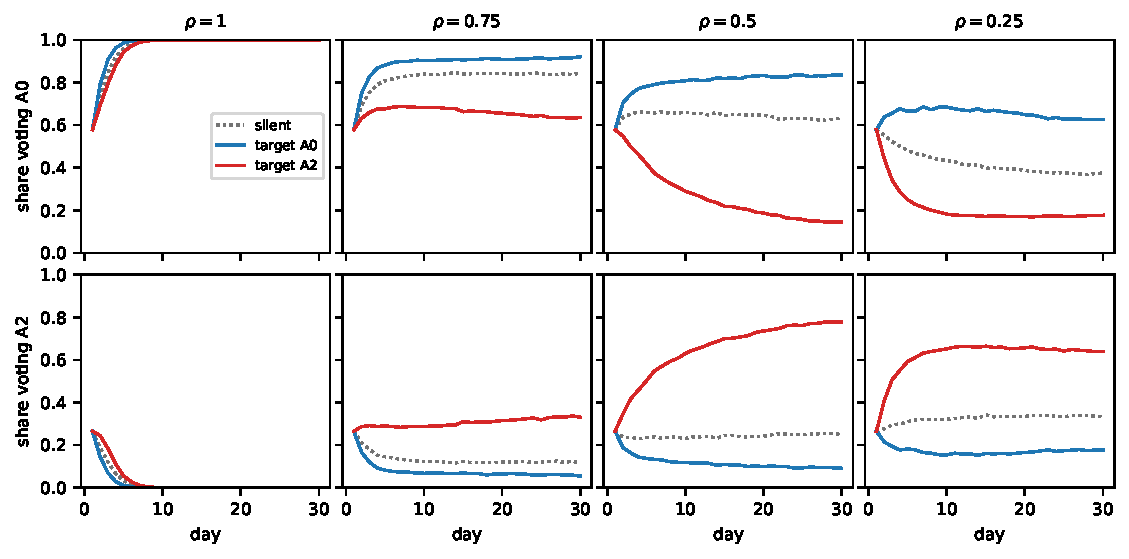
\includegraphics[width=0.95\linewidth]{figures/fig_votes.pdf}
\caption{Share of agents voting A0 (top) and A2 (bottom) at the end of each day, Eq.~(\ref{eq:share}), without a
controller (dotted), with the controller targeting A0 (blue) and A2 (red); one column per memory $\rho$. $q = 6$,
$q_c = 12$, $b = 1$, gate on. Day 0: nobody has voted yet, every share is 0. 95\% intervals are narrower than the
lines ($\pm 0.01$).}
\label{fig:votes}
\end{figure}

\begin{itemize}\itemsep1pt
\item \textbf{The shorter the memory, the less firmly the silent swarm holds the truth}: 100\%, 85\%, 63\% and
  38\% vote A0 on day 30 for $\rho = 1, 0.75, 0.5, 0.25$.
\item \textbf{With full memory no controller matters}: every agent votes A0 by day $\approx 8$ in all three arms.
\item \textbf{The false controller wins the majority when $\rho \le 0.5$}: A2 gets 78\% ($\rho = 0.5$) and 64\%
  ($\rho = 0.25$) of the votes, against 25\% and 33\% in silence; at $\rho = 0.75$ only 33\%.
\item \textbf{The truth controller restores the truth} to 92\% ($\rho = 0.75$) and 84\% ($\rho = 0.5$), but only to
  63\% at $\rho = 0.25$.
\end{itemize}

\section{Paired susceptibility over time}

\begin{figure}[H]
\centering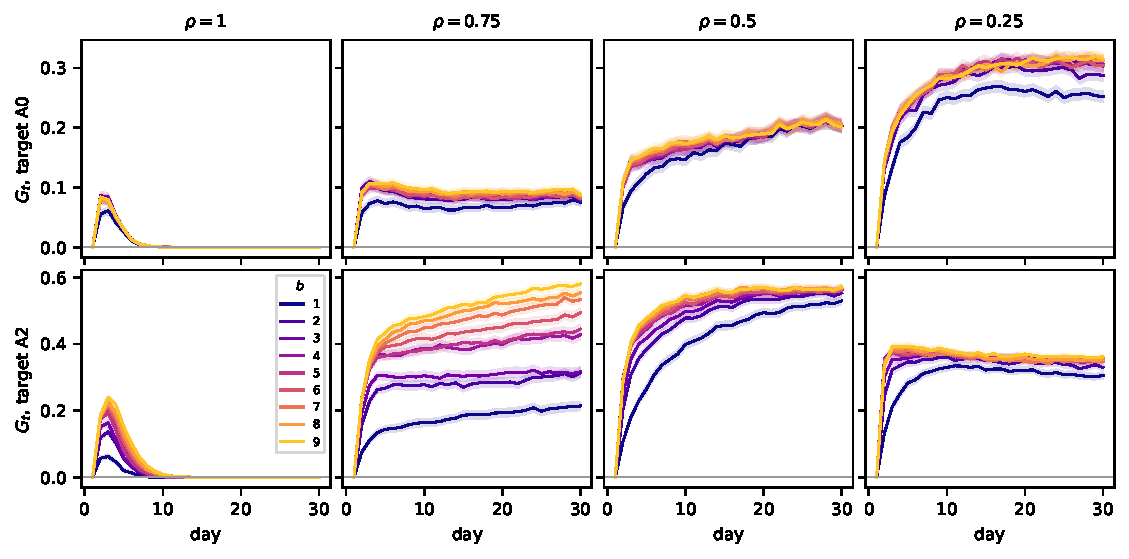
\includegraphics[width=0.95\linewidth]{figures/fig_gain_time.pdf}
\caption{Paired susceptibility $G_t$, Eq.~(\ref{eq:chi}), target A0 (top) and A2 (bottom), one curve per
budget $b$; $q = 6$, $q_c = 12$, gate on. $G_0 = 0$: before the first day the three arms are identical. Bands: 95\%
intervals.}
\label{fig:gaintime}
\end{figure}

\begin{itemize}\itemsep1pt
\item \textbf{Susceptibility peaks at intermediate memory}: on day 30, target A2, $G = 0.22$--$0.58$
  ($\rho = 0.75$), $0.53$--$0.57$ ($\rho = 0.5$), $0.31$--$0.36$ ($\rho = 0.25$); target A0, $0.08$--$0.09$,
  $0.20$, $0.25$--$0.32$.
\item \textbf{With full memory control is only transient}: target A2 reaches $0.24$ on day 3 ($b = 9$) and is
  gone by day $\approx 12$.
\item \textbf{The budget matters only when agents remember well}: at $\rho = 0.75$, target A2 grows from $0.22$
  ($b = 1$) to $0.58$ ($b = 9$); at $\rho \le 0.5$ every $b \ge 2$ gives about the same.
\item \textbf{With heavy forgetting a large budget overshoots}: at $\rho = 0.25$, $b = 9$, target A2 peaks at
  $0.39$ (day 5) and settles at $0.36$.
\end{itemize}

\section{Phase diagrams of the susceptibility}

\begin{figure}[H]
\centering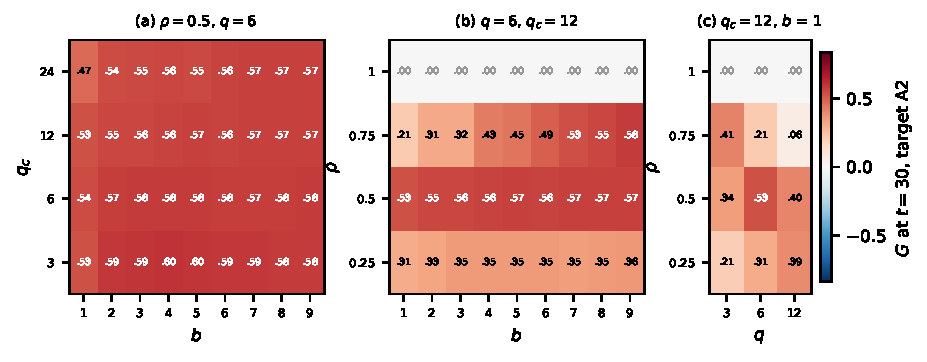
\includegraphics[width=0.98\linewidth]{figures/fig_phase_gain.pdf}
\caption{$G$ on day 30, target A2, gate on: (a) over the posts the controller reads $q_c$ and the budget $b$, at
$\rho = 0.5$, $q = 6$; (b) over $\rho$ and $b$, at $q = 6$, $q_c = 12$; (c) over $\rho$ and the posts each agent
reads $q$, at $q_c = 12$, $b = 1$. Grey number: the 95\% interval includes 0. Same colour scale as in the
Simulation 2 report.}
\label{fig:phasegain}
\end{figure}

\begin{itemize}\itemsep1pt
\item \textbf{Memory is the main axis} (panel b): $G = 0$ at $\rho = 1$, largest at $\rho = 0.5$ (0.53--0.57),
  and at $\rho = 0.75$ only with a large budget.
\item \textbf{At $\rho = 0.5$ the budget and $q_c$ hardly matter} (panel a: 0.47--0.60; mean 0.58, 0.57, 0.56,
  0.55 for $q_c = 3, 6, 12, 24$).
\item \textbf{Reading more defends the proof only when agents remember well} (panel c): at $\rho = 0.75$, $G$
  falls from $0.41$ ($q = 3$) to $0.06$ ($q = 12$); at $\rho = 0.25$ it rises from $0.21$ to $0.40$. A likely
  reason, not tested: with heavy forgetting the proof cannot be rebuilt anyway, and reading more only spreads the
  controller's facts faster.
\end{itemize}

\section{Susceptibility against the budget, and its slope}

\begin{figure}[H]
\centering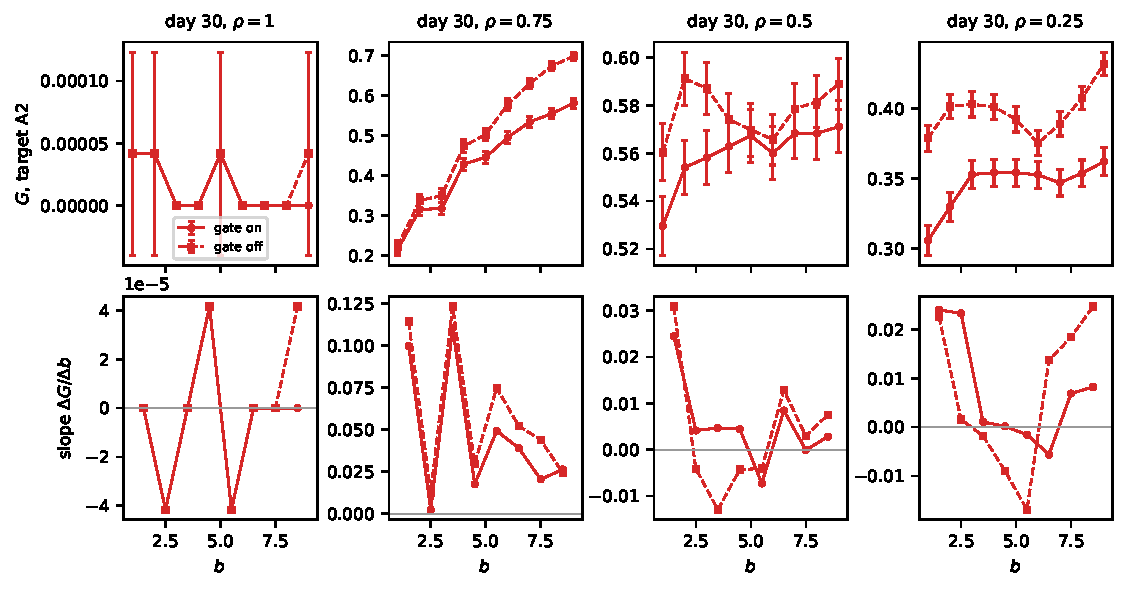
\includegraphics[width=0.95\linewidth]{figures/fig_gain_strength.pdf}
\caption{Top: $G$ on day 30, target A2, against the budget $b$, one panel per $\rho$; gate on (solid) and off
(dashed); bars: 95\% intervals. Bottom: the slope between neighbouring budgets, Eq.~(\ref{eq:slope}). (Simulation 1
has a single end point, so all four $\rho$ are shown; Simulation 2 shows $t = 5$ and $t = 30$.)}
\label{fig:strength}
\end{figure}

\begin{itemize}\itemsep1pt
\item \textbf{When agents remember well, more budget keeps buying susceptibility}: at $\rho = 0.75$ the slope is
  $0.10$ for the first extra fact per night and still $0.04$ on average after it.
\item \textbf{When they forget, one fact per night is almost enough}: at $\rho = 0.5$ and $0.25$ the slope is
  $0.02$ for the first step and about $0.002$ after it.
\item \textbf{The marginal susceptibility is the efficiency of adding budget}: worth paying for only at
  $\rho = 0.75$.
\item \textbf{Turning the gate off adds susceptibility where the budget matters}: up to $+0.12$ at $\rho = 0.75$
  ($0.70$ against $0.58$ at $b = 9$), $+0.02$ to $+0.07$ at $\rho = 0.25$.
\end{itemize}

\section{Susceptibility per fact posted}

\begin{figure}[H]
\centering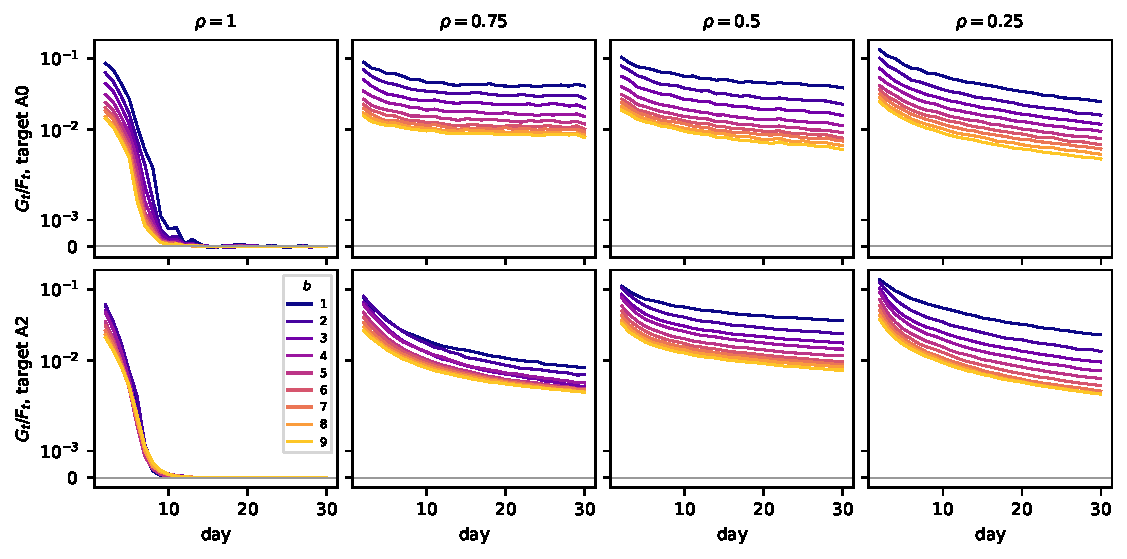
\includegraphics[width=0.95\linewidth]{figures/fig_gain_per_fact.pdf}
\caption{Gain per fact $G_t/F_t$ (log scale) for target A0 (top) and A2 (bottom), one curve per budget; $q = 6$,
$q_c = 12$, gate on. Shown once the controller has posted at least half a fact on average.}
\label{fig:perfact}
\end{figure}

\begin{itemize}\itemsep1pt
\item \textbf{The smallest budget gets the most per fact}: on day 30, target A2, $\rho = 0.5$: $0.036$ per fact at
  $b = 1$ (15 facts) against $0.007$ at $b = 9$ (77 facts); at $\rho = 0.25$: $0.023$ against $0.003$.
\item \textbf{When agents remember well every fact buys little} ($\rho = 0.75$: $0.008$ at $b = 1$, $0.004$ at
  $b = 9$), because the proof keeps pulling the swarm back.
\item \textbf{The truth controller gets the most per fact at small budgets} ($0.039$ at $\rho = 0.5$, $b = 1$): the
  gate keeps it silent once the swarm agrees, so it posts only 2--10 facts.
\end{itemize}

\section{Who holds the proof}

\begin{figure}[H]
\centering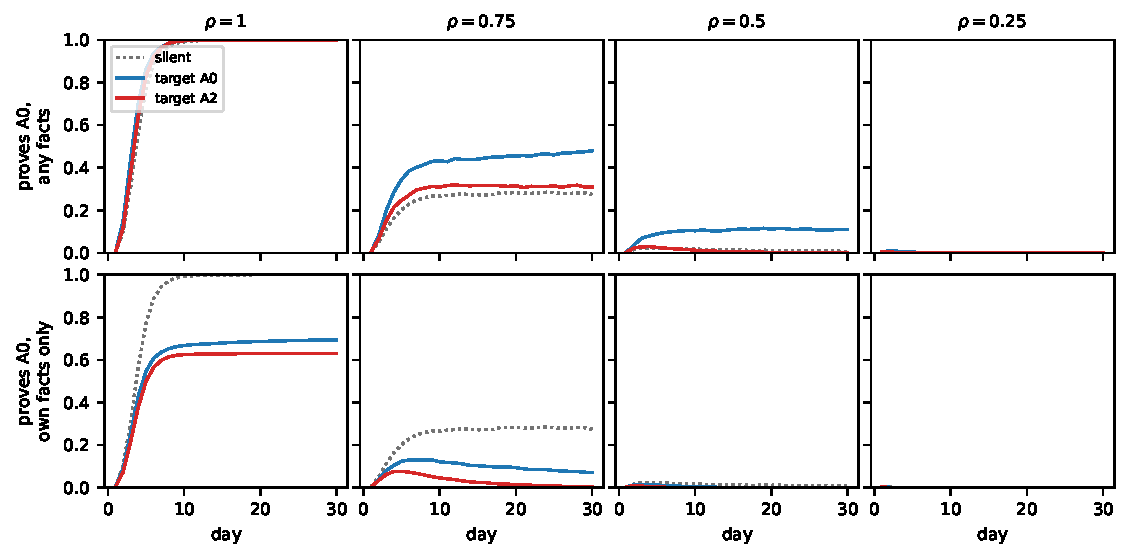
\includegraphics[width=0.95\linewidth]{figures/fig_proofs.pdf}
\caption{Share of agents whose remembered facts prove A0 (top) and prove it from the agents' original facts only
(bottom); silent (dotted), target A0 (blue), target A2 (red); $q = 6$, $q_c = 12$, $b = 1$, gate on.}
\label{fig:proofs}
\end{figure}

\begin{itemize}\itemsep1pt
\item \textbf{Proofs need memory}: on day 30 the silent swarm has 100\%, 28\%, 1\% and 0\% of agents proving A0
  for $\rho = 1, 0.75, 0.5, 0.25$. Below $\rho = 0.75$ votes rest on beliefs, not proofs.
\item \textbf{Every controller replaces the agents' own proofs}: with full memory all agents prove A0 under any
  arm, but only 69\% (target A0) and 63\% (target A2) from their own facts (100\% in silence); at $\rho = 0.75$,
  48\% prove A0 under the truth controller but only 7\% from their own facts.
\item \textbf{The false controller's true facts complete proofs of A0} (31\% against 28\% in silence at
  $\rho = 0.75$), while own-evidence proofs fall to 0.5\%.
\end{itemize}

\section{Readability over time}

\begin{figure}[H]
\centering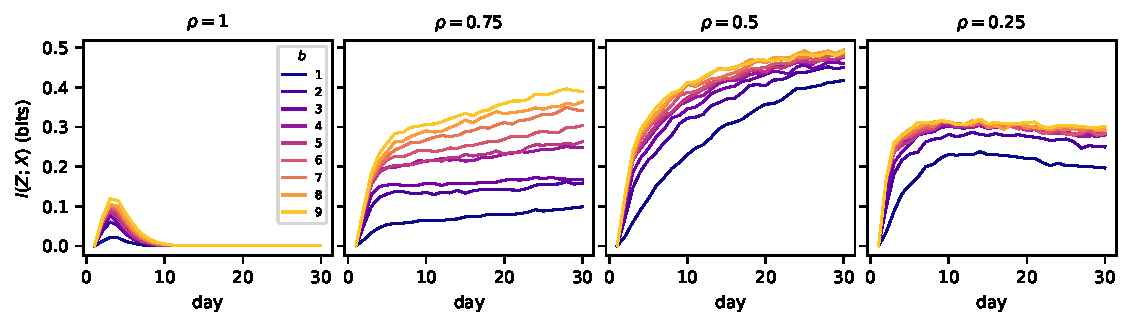
\includegraphics[width=0.95\linewidth]{figures/fig_I_time.pdf}
\caption{Readability $I(Z;X)$, Eq.~(\ref{eq:I}), with $X$ one agent's vote, one curve per budget; $q = 6$,
$q_c = 12$, gate on.}
\label{fig:Itime}
\end{figure}

\begin{itemize}\itemsep1pt
\item \textbf{The target is most readable at intermediate memory}: on day 30, $I = 0.10$--$0.39$ bits
  ($\rho = 0.75$), $0.42$--$0.49$ ($\rho = 0.5$), $0.20$--$0.30$ ($\rho = 0.25$), 0 ($\rho = 1$).
\item \textbf{The budget orders the curves}: larger budgets are more readable, strongly at $\rho = 0.75$
  ($0.10 \to 0.39$), weakly elsewhere.
\item \textbf{With full memory the target is readable only for a few days}: $I$ peaks at $0.12$ bits on day 3
  ($b = 9$).
\end{itemize}

\section{Efficiency over time}

\begin{figure}[H]
\centering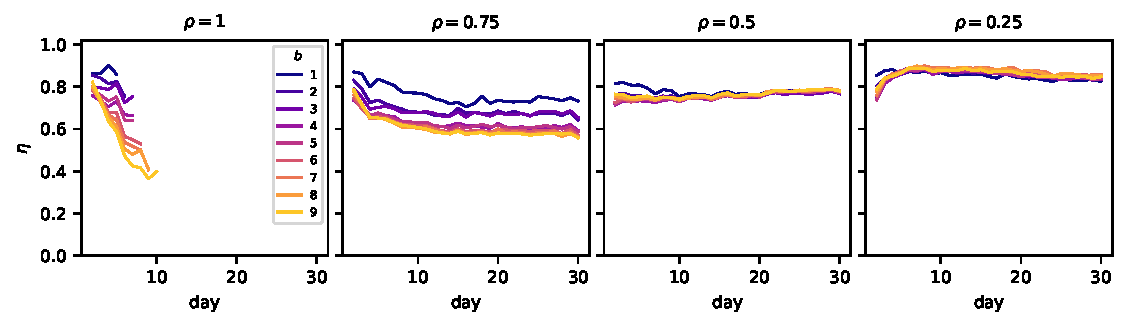
\includegraphics[width=0.95\linewidth]{figures/fig_eta_time.pdf}
\caption{Efficiency $\eta = I/C$, Eq.~(\ref{eq:eta}), one agent's vote, one curve per budget; $q = 6$, $q_c = 12$,
gate on. Blank: undefined ($C < 0.01$ bits). Pseudo-count, Eq.~(\ref{eq:smooth}).}
\label{fig:etatime}
\end{figure}

\begin{itemize}\itemsep1pt
\item \textbf{Efficiency is high when agents forget}: on day 30, $\eta = 0.77$--$0.78$ ($\rho = 0.5$),
  $0.82$--$0.86$ ($\rho = 0.25$), flat across budgets.
\item \textbf{When they remember well it falls with the budget}: $0.73$ at $b = 1$ to $0.56$ at $b = 9$
  ($\rho = 0.75$): the false controller grows with $b$ while the truth controller is near its ceiling, so the pair
  turns lopsided.
\item \textbf{With full memory $\eta$ is defined only for the first days}, before the controllers' effects vanish.
\end{itemize}

\section{Phase diagrams of the readability}

\begin{figure}[H]
\centering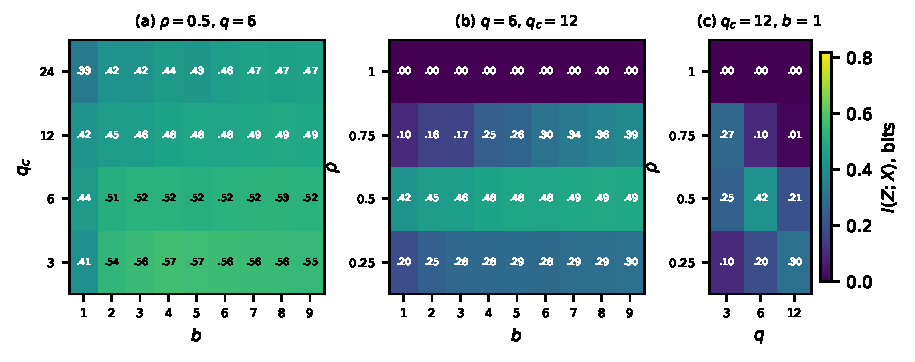
\includegraphics[width=0.98\linewidth]{figures/fig_phase_I.pdf}
\caption{$I(Z;X)$ on day 30, one agent's vote, gate on; panels as in Figure~\ref{fig:phasegain}.}
\label{fig:phaseI}
\end{figure}

\begin{itemize}\itemsep1pt
\item \textbf{Readability follows the susceptibility}: highest at $\rho = 0.5$ (0.42--0.49 bits; up to 0.57 in
  panel a), 0 at $\rho = 1$.
\item \textbf{The posts each agent reads have the same reversal as $G$} (panel c): at $\rho = 0.75$, $I$ falls from
  $0.27$ ($q = 3$) to $0.01$ ($q = 12$); at $\rho = 0.25$ it rises from $0.10$ to $0.30$.
\item \textbf{At $\rho = 0.75$ the budget sets it} (panel b: $0.10 \to 0.39$ from $b = 1$ to 9).
\end{itemize}

\section{Phase diagrams of the efficiency}

\begin{figure}[H]
\centering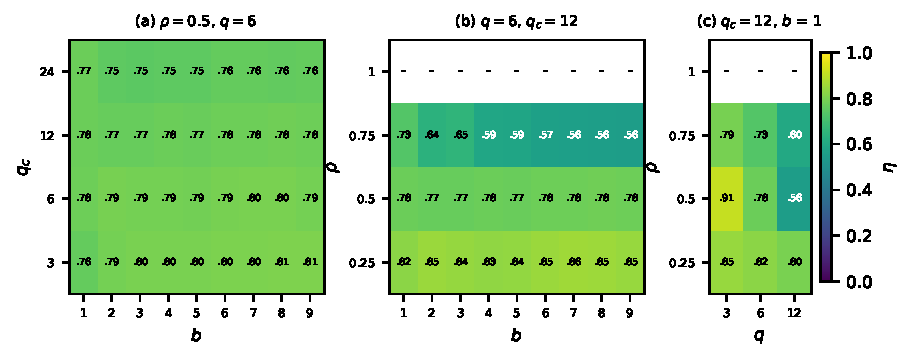
\includegraphics[width=0.98\linewidth]{figures/fig_phase_eta.pdf}
\caption{$\eta$ on day 30, one agent's vote, gate on; panels as in Figure~\ref{fig:phasegain}. Dash: undefined.}
\label{fig:phaseeta}
\end{figure}

\begin{itemize}\itemsep1pt
\item \textbf{Efficiency is high and fairly uniform} (0.75--0.81 in panel a), except at $\rho = 0.75$ with a large
  budget (down to 0.56, panel b).
\item \textbf{It is lowest where the pair is most lopsided}, not where control is weakest: $\eta$ measures how
  mirror-like the two controllers' changes are; the size is $I$ (Figure~\ref{fig:phaseI}).
\end{itemize}

\section{Conclusions}

\begin{enumerate}\itemsep2pt
\item \textbf{Memory decides whether a swarm that owns a proof can be steered.} With full memory every effect
  vanishes within about ten days. As memory shortens the silent swarm holds the truth less firmly (100\%, 85\%, 63\%,
  38\% voting A0 on day 30) and the controllers' susceptibility rises, peaking at $\rho = 0.5$.
\item \textbf{Heavy forgetting weakens both controllers.} At $\rho = 0.25$ the false controller gains less than at
  $\rho = 0.5$ and the truth controller restores only 63\% of votes to A0: facts fade before they accumulate.
\item \textbf{More budget pays only when agents remember well} ($\rho = 0.75$: slope 0.10, then 0.04 per extra
  fact per night). Elsewhere one fact per night is almost enough, and the smallest budget is the most effective per
  fact.
\item \textbf{The posts each agent reads switch sides with memory}: they defend the proof at $\rho = 0.75$ and help
  the controller at $\rho = 0.25$.
\item \textbf{Control replaces the agents' own proofs}, even when every agent ends up proving the truth.
\item \textbf{Readability tracks susceptibility; efficiency tracks symmetry.} $I$ ranges from 0 to 0.57 bits; $\eta$
  stays at 0.56--0.91 and falls only where one controller grows much more than the other.
\item \textbf{Compared with Simulation 2} (same settings, about the same facts posted): Simulation 1 is more
  susceptible at $\rho = 0.5$ (0.53 against 0.33, target A2) and less at $\rho = 0.25$ (0.31 against 0.43), and its
  vote gate matters far more.
\end{enumerate}

\appendix
\section{Gate off}\label{app:gateoff}

\begin{figure}[H]
\centering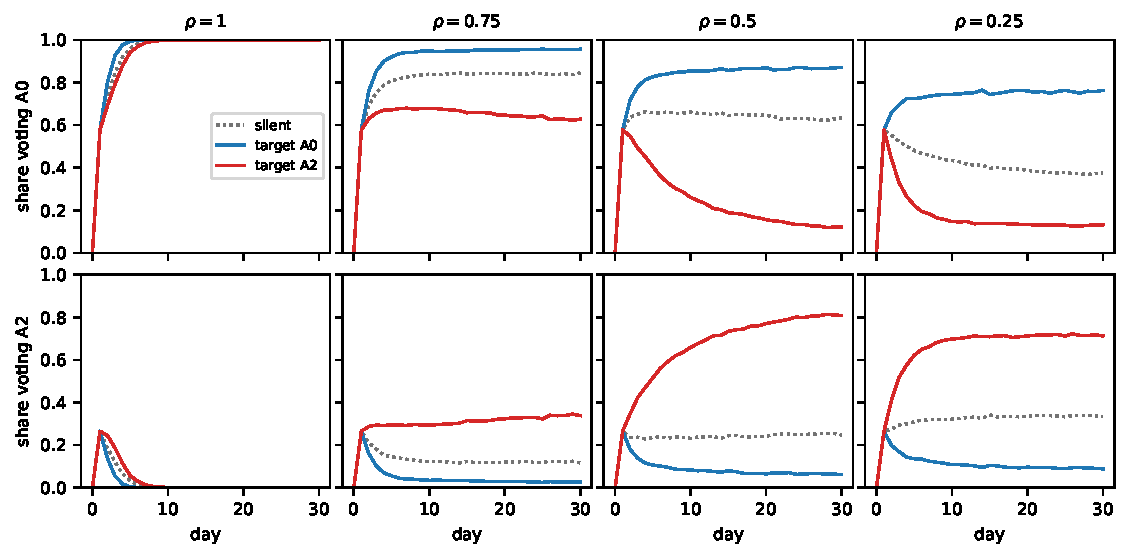
\includegraphics[width=0.95\linewidth]{figures/fig_votes_gateoff.pdf}
\caption{As Figure~\ref{fig:votes}, gate off.}
\label{fig:votesoff}
\end{figure}

\begin{figure}[H]
\centering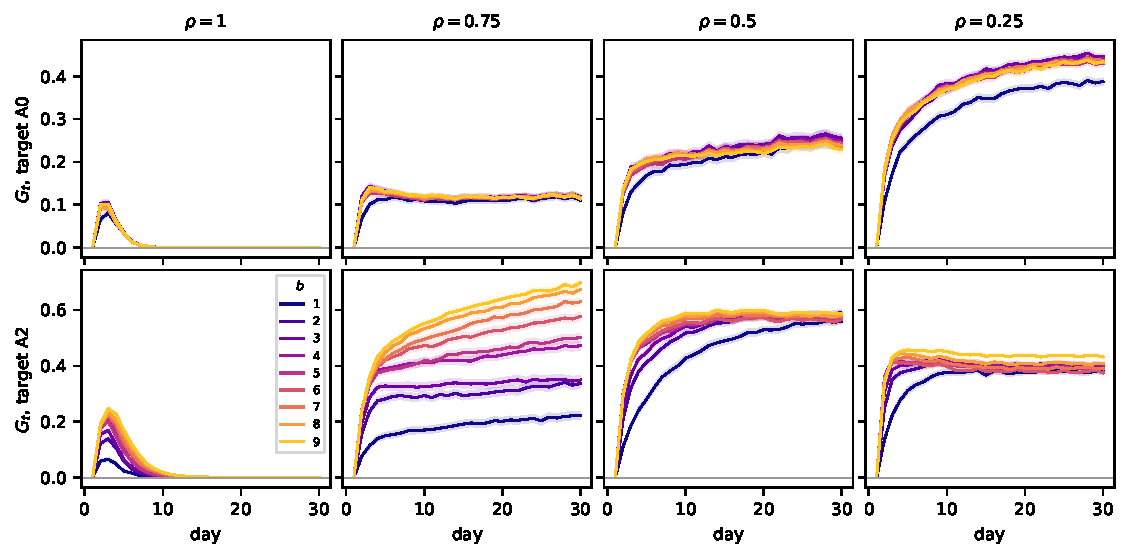
\includegraphics[width=0.95\linewidth]{figures/fig_gain_time_gateoff.pdf}
\caption{As Figure~\ref{fig:gaintime}, gate off.}
\label{fig:gaintimeoff}
\end{figure}

\begin{figure}[H]
\centering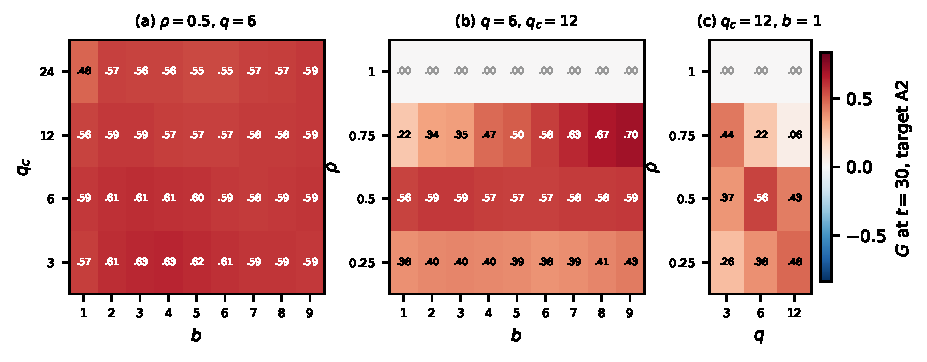
\includegraphics[width=0.98\linewidth]{figures/fig_phase_gain_gateoff.pdf}
\caption{As Figure~\ref{fig:phasegain}, gate off.}
\label{fig:phasegainoff}
\end{figure}

\begin{figure}[H]
\centering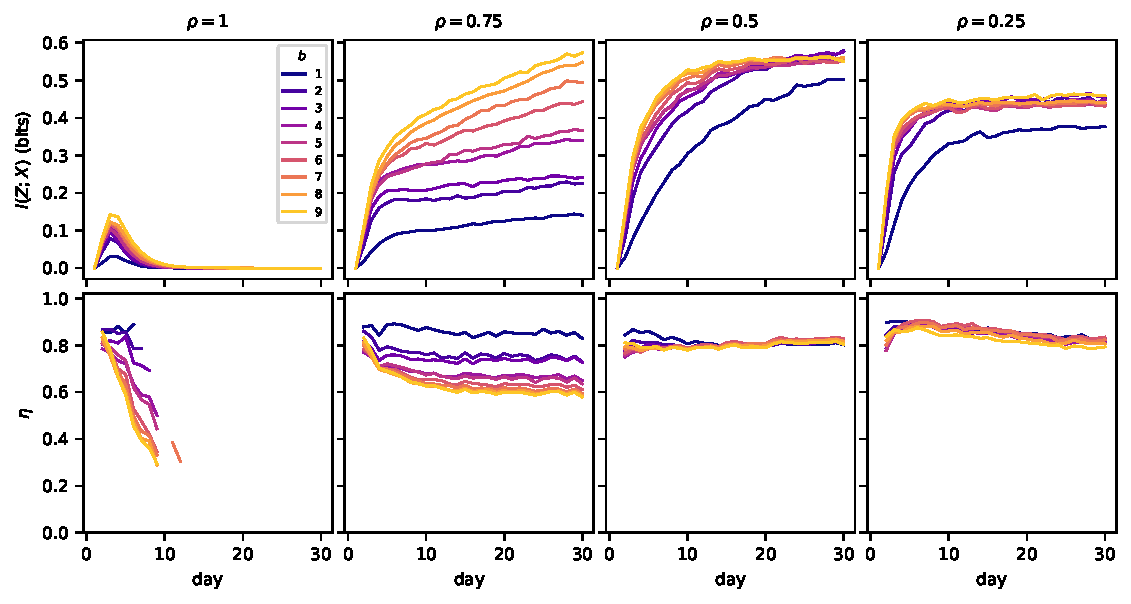
\includegraphics[width=0.95\linewidth]{figures/fig_Ieta_time_vote_gateoff.pdf}
\caption{As Figures~\ref{fig:Itime} (top) and \ref{fig:etatime} (bottom), gate off.}
\label{fig:infooff}
\end{figure}

\begin{figure}[H]
\centering
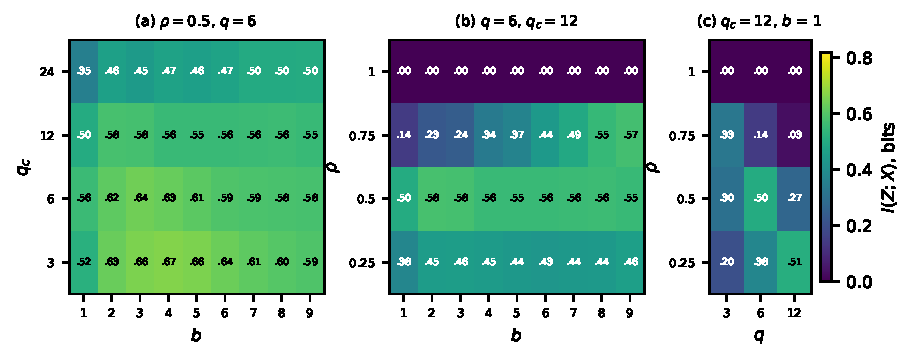
\includegraphics[width=0.98\linewidth]{figures/fig_phase_I_gateoff.pdf}\\
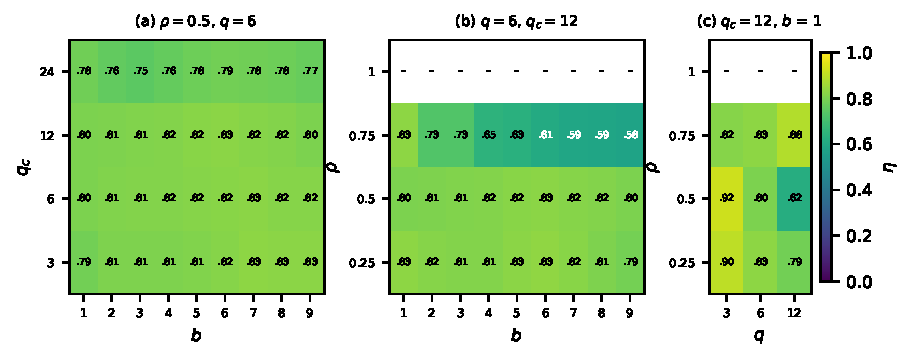
\includegraphics[width=0.98\linewidth]{figures/fig_phase_eta_gateoff.pdf}
\caption{As Figures~\ref{fig:phaseI} (top) and \ref{fig:phaseeta} (bottom), gate off.}
\label{fig:phaseinfooff}
\end{figure}

\begin{itemize}\itemsep1pt
\item \textbf{The gate matters much more than in Simulation 2}: with it off, the controller posts 43--98 more
  facts per episode ($\rho < 1$), and $G$ on day 30 rises by up to $+0.12$ (target A2, most at $\rho = 0.75$) and by
  $+0.03$ to $+0.16$ (target A0, most at $\rho = 0.25$).
\item \textbf{Readability rises with it} ($+0.08$ to $+0.16$ bits on average by $\rho$), efficiency changes by at most
  $0.05$.
\end{itemize}

\section{Other states}\label{app:states}

\begin{figure}[H]
\centering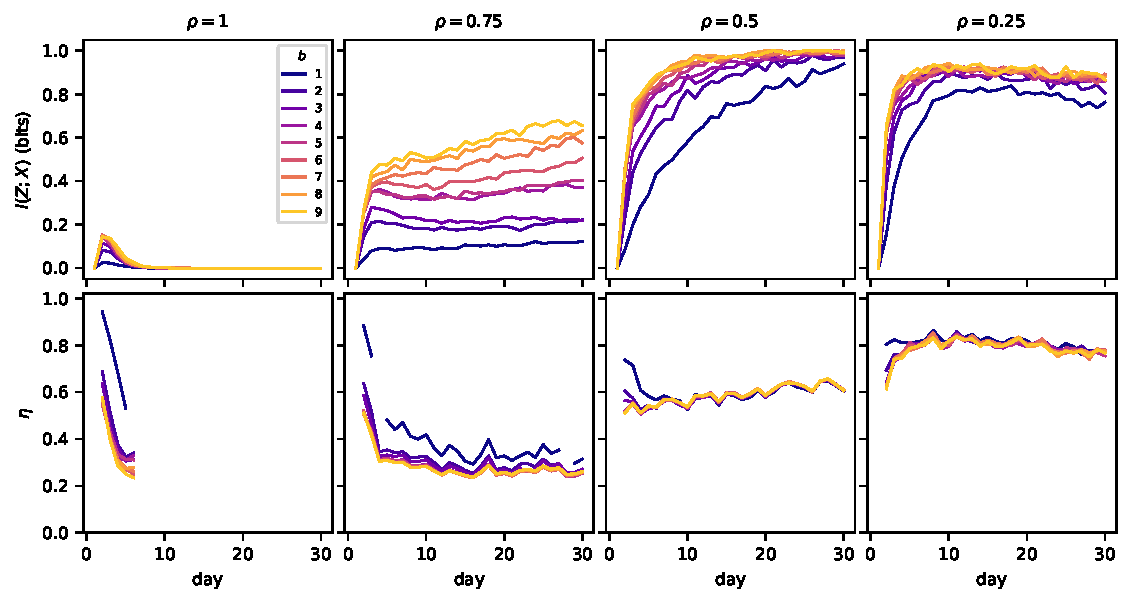
\includegraphics[width=0.95\linewidth]{figures/fig_Ieta_time_plur.pdf}
\caption{Readability (top) and efficiency (bottom) over time with $X$ = the plurality of the votes; layout as in
Figures~\ref{fig:Itime} and \ref{fig:etatime}.}
\label{fig:plurtime}
\end{figure}

\begin{figure}[H]
\centering
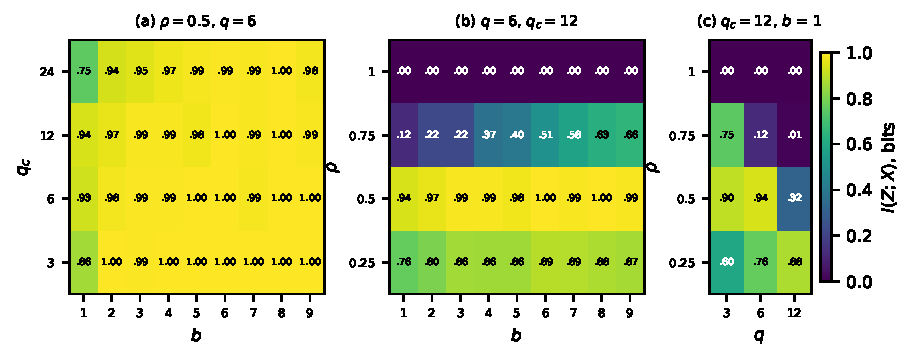
\includegraphics[width=0.98\linewidth]{figures/fig_phase_I_plur.pdf}\\
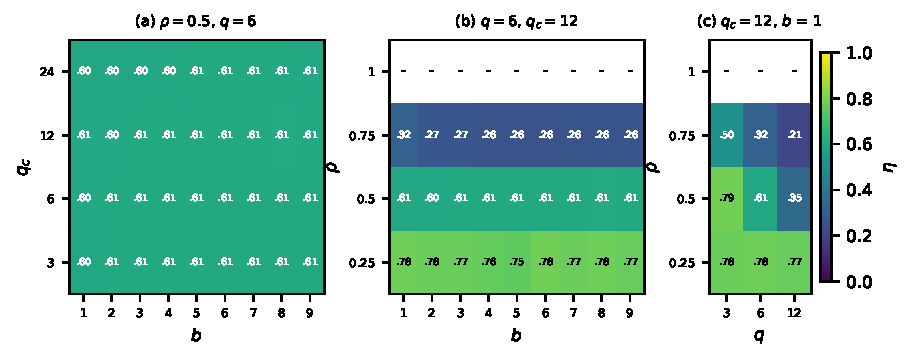
\includegraphics[width=0.98\linewidth]{figures/fig_phase_eta_plur.pdf}
\caption{Readability (top) and efficiency (bottom) on day 30, plurality; panels as in Figure~\ref{fig:phasegain}.}
\label{fig:plurphase}
\end{figure}

\begin{figure}[H]
\centering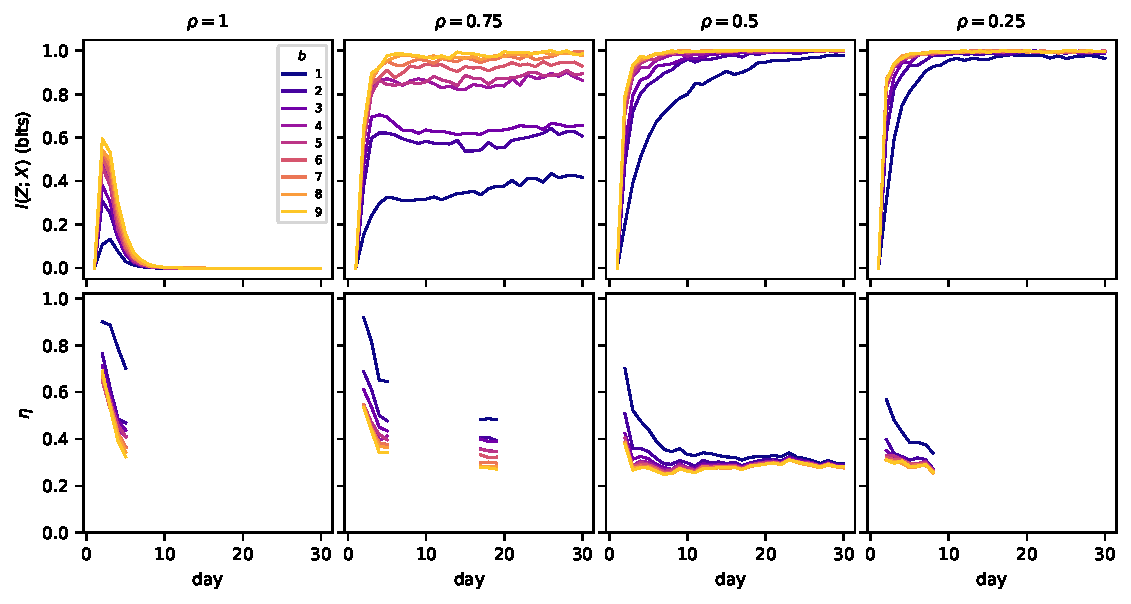
\includegraphics[width=0.95\linewidth]{figures/fig_Ieta_time_s1.pdf}
\caption{As Figure~\ref{fig:plurtime}, with $X$ = S1.}
\label{fig:s1time}
\end{figure}

\begin{figure}[H]
\centering
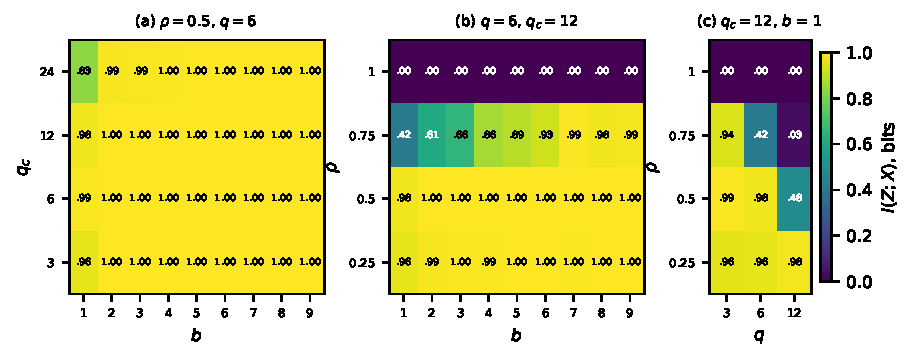
\includegraphics[width=0.98\linewidth]{figures/fig_phase_I_s1.pdf}\\
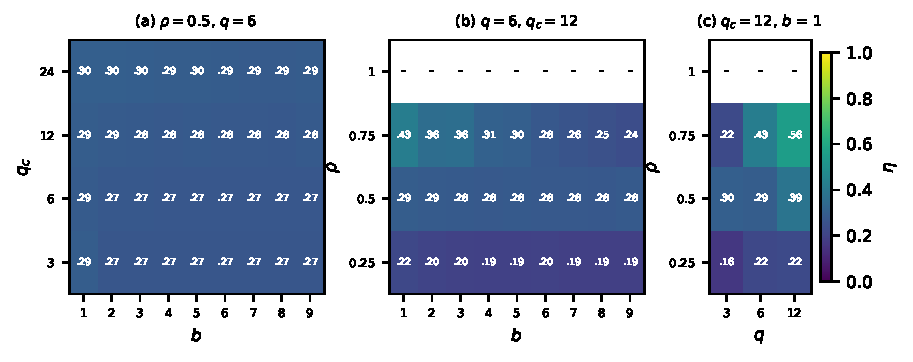
\includegraphics[width=0.98\linewidth]{figures/fig_phase_eta_s1.pdf}
\caption{As Figure~\ref{fig:plurphase}, S1.}
\label{fig:s1phase}
\end{figure}

\begin{figure}[H]
\centering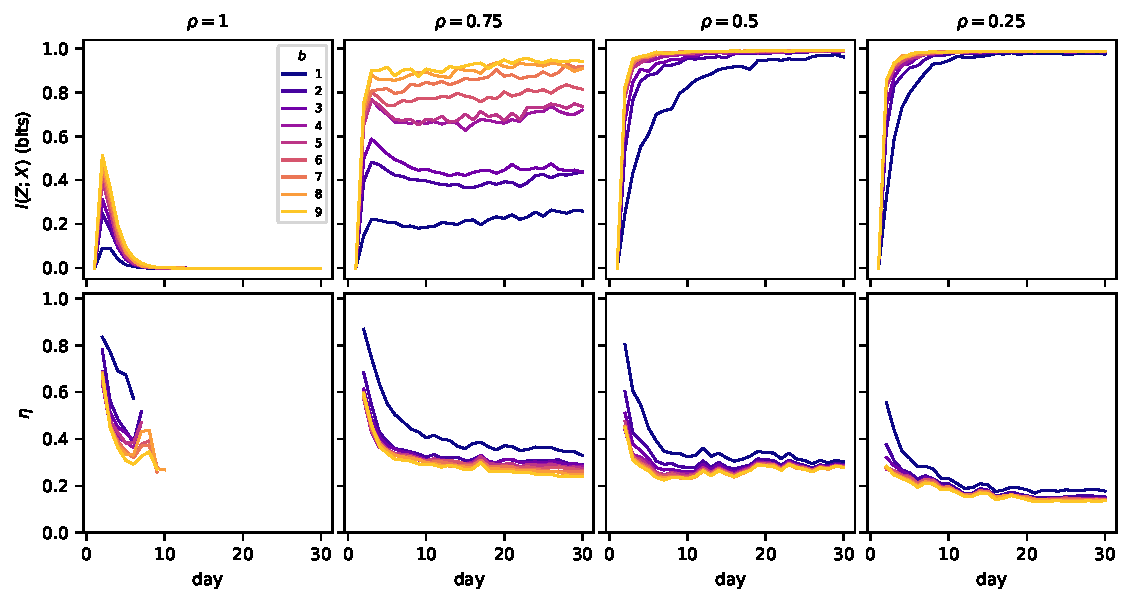
\includegraphics[width=0.95\linewidth]{figures/fig_Ieta_time_s3.pdf}
\caption{As Figure~\ref{fig:plurtime}, with $X$ = S3.}
\label{fig:s3time}
\end{figure}

\begin{figure}[H]
\centering
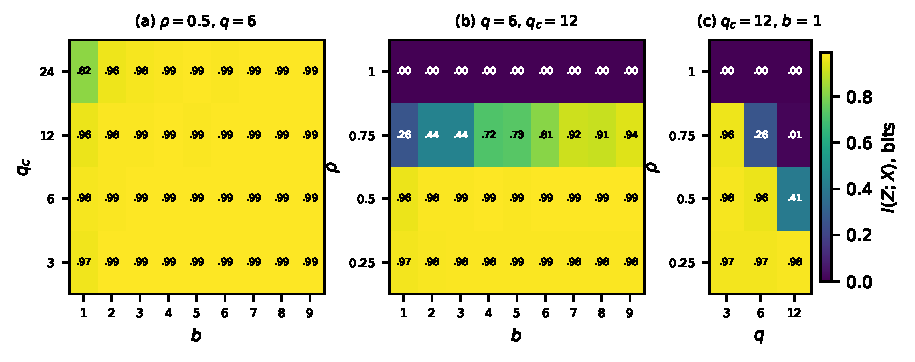
\includegraphics[width=0.98\linewidth]{figures/fig_phase_I_s3.pdf}\\
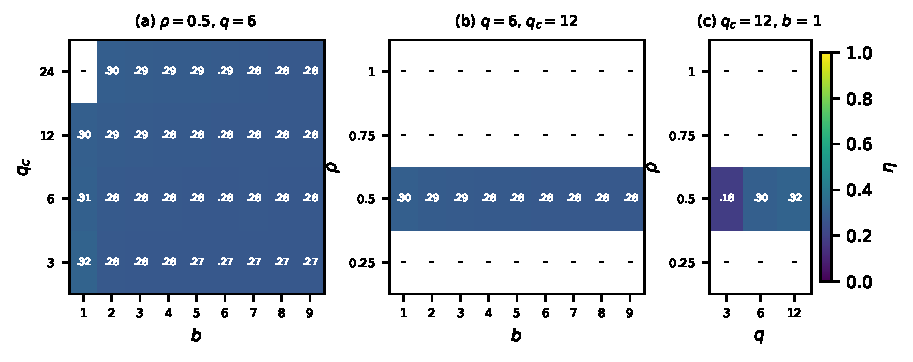
\includegraphics[width=0.98\linewidth]{figures/fig_phase_eta_s3.pdf}
\caption{As Figure~\ref{fig:plurphase}, S3.}
\label{fig:s3phase}
\end{figure}

\begin{itemize}\itemsep1pt
\item \textbf{Swarm-level states read far more than one agent's vote}: at $\rho = 0.5$, day 30, main setting,
  $I = 0.42$ (one vote), $0.93$ (plurality), $0.97$ (S1), $0.96$ (S3) bits; at $\rho = 0.25$, $0.20$, $0.76$,
  $0.96$, $0.97$.
\item \textbf{But their efficiency is lower}: on day 30, main setting, $\eta = 0.32$--$0.78$ (plurality),
  $0.22$--$0.43$ (S1), $0.18$--$0.33$ (S3), against $0.73$--$0.82$ for one vote. Without the pseudo-count of
  Eq.~(\ref{eq:smooth}), $C$ would be infinite for S1 and S3 in many settings. The plurality's $\eta$ is noisier than
  one vote's because silence rarely lets A2 win at $\rho = 0.75$, so a few episodes set that cell.
\item \textbf{Belief-based states (S1, S3) read the most}, likely because beliefs move before votes do and without
  the noise of the vote draw. The plurality is the swarm state built from votes alone.
\end{itemize}

\section{Strong control}\label{app:strong}

\begin{figure}[H]
\centering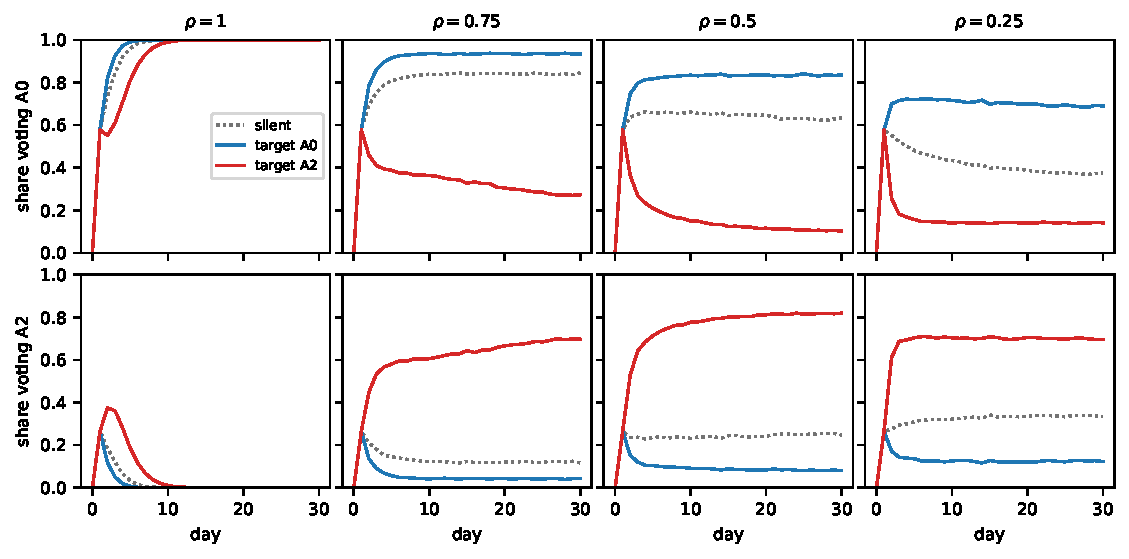
\includegraphics[width=0.95\linewidth]{figures/fig_votes_strong.pdf}
\caption{As Figure~\ref{fig:votes}, at the largest budget $b = 9$.}
\label{fig:votesstrong}
\end{figure}

\begin{figure}[H]
\centering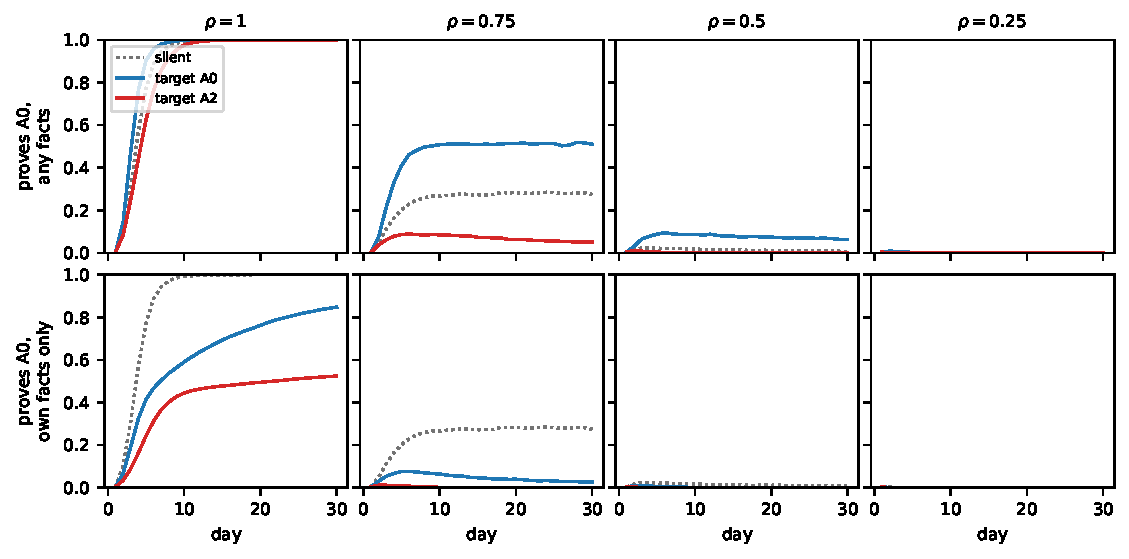
\includegraphics[width=0.95\linewidth]{figures/fig_proofs_strong.pdf}
\caption{As Figure~\ref{fig:proofs}, at $b = 9$.}
\label{fig:proofsstrong}
\end{figure}

\begin{itemize}\itemsep1pt
\item \textbf{A large budget doubles the false controller's share when agents remember well}: target A2 gets 70\%
  of votes at $\rho = 0.75$ (33\% at $b = 1$); at $\rho = 0.5$ and $0.25$, 82\% and 70\% (78\% and 64\% at $b = 1$).
\item \textbf{The truth controller gains little from it}: A0 at 93\%, 84\%, 69\% (92\%, 84\%, 63\% at $b = 1$).
\item \textbf{Proofs from own facts vanish}: at $\rho = 0.75$, 2.6\% (target A0) and 0\% (target A2) against 28\%
  in silence.
\end{itemize}

\paragraph{Caveats.} One world, 24 exact-Bayesian agents voting by probability matching, one controller policy
posting a fixed batch each night; 1{,}000 episodes per setting (95\% intervals on $G$ about $\pm0.02$).
Information is plug-in from 1{,}000 episodes per arm. Data:
\texttt{results/simulation\_1/2026-10-15\_sim1\_pm\_symmetric\_fine}; tables and figures:
\texttt{analysis/task003\_llm\_free/shared\_analysis/gold\_standard/}.

\end{document}
